\documentclass[11pt]{article}
\usepackage[utf8]{inputenc} % Para caracteres en espa�ol
\usepackage{amsmath,amsthm,amsfonts,amssymb,amscd}
\usepackage{multirow,booktabs}
\usepackage[table]{xcolor}
\usepackage{fullpage}
\usepackage{lastpage}
\usepackage{enumitem}
\usepackage{multicol}
\usepackage{fancyhdr}
\usepackage{mathrsfs}
\usepackage{pdfpages}
\usepackage{wrapfig}
\usepackage{setspace}
\usepackage{esvect}
\usepackage{calc}
\usepackage{multicol}
\usepackage{cancel}
\usepackage{graphicx}
\graphicspath{ {} }
\usepackage[retainorgcmds]{IEEEtrantools}
\usepackage[margin=3cm]{geometry}
\usepackage{amsmath}
\newlength{\tabcont}
\setlength{\parindent}{0.0in}
\setlength{\parskip}{0.05in}
\usepackage{empheq}
\usepackage{framed}
\usepackage[most]{tcolorbox}
\usepackage{xcolor}
\colorlet{shadecolor}{orange!15}
\parindent 0in
\parskip 12pt
\geometry{margin=1in, headsep=0.25in}
\theoremstyle{definition}
\newtheorem{defn}{Definition}
\newtheorem{reg}{Rule}
\newtheorem{exer}{Exercise}

% Two more packages that make it easy to show MATLAB code
\usepackage[T1]{fontenc}
\usepackage[framed,numbered]{matlab-prettifier}
\lstset{
	style = Matlab-editor,
	basicstyle=\mlttfamily\small,
}

\newtheorem{note}{Note}
\begin{document}
\begin{lstlisting}
function hw8p1
r = 0.05; %Chamber Radius [m]
l = 0.15; % Chamber Length [m]
A = pi*r^2; %Grid Area [m^2]
A_a = pi*r^2 + 2*pi*r*l; %Anode Area [m^2]
T_g = 0.8; %Grid Transparency
n_o = 10^18; %Neutral Particle Density [m^-3]
V = A*l; % Volume [m^3]
Ui = 12.13;% Ionization Potential [eV]
Ue = 10; % Excitation Potential [eV]
m =9.10938e-31;
M = 2.18e-25;

k = 1.38064852e-23; % Boltzmann Constant [J/K]
k2 = 8.6173303e-5; % Boltzmann Constant [eV/K]

Te = [3 3.5 4 4.5 5 5.5 6 6.5 7 7.5 8 8.5 9 9.5 10]; % Electron Temperature [eV]
OVi = [1.08e-15 2.13e-15 3.59e-15 5.43e-15 7.61e-15 1.01e-14 1.28e-14 1.57e-14 1.88e-14 2.20e-14 2.53e-14 2.86e-14 3.20e-14 3.55e-14 3.90e-14];% Ionization Rate Coefficient [m^3/s]
OVe = [2.66e-15 4.66e-15 7.12e-15 9.93e-15 1.30e-14 1.61e-14 1.94e-14 2.26e-14 2.57e-14 2.87e-14 3.14e-14 3.34e-14 3.41e-14 3.21e-14 2.48e-14];% Excitation Rate Coefficient [m^3/s]

for i = 1:length(Te)
    v_a = sqrt(((k/k2)*Te(i))/M);
    eta_d(i) = (((2*n_o*OVi(i)*V)/(T_g*A*v_a))*(Ui + (OVe(i)/OVi(i))*Ue))+((1/(T_g))*(2.5*Te(i) + 2*Te(i)*log((A_a/A)*sqrt((2*M)/(m*pi)))));
end

plot(Te,eta_d,'linewidth',2)
title('Discharge Loss V. Electron Temperature')
ylabel('Discharge Loss (eV/ion)')
xlabel('Electron Temperature [eV]')
grid on
grid minor

set(gcf,'paperorientation','landscape');
set(gcf,'paperunits','normalized');
set(gcf,'paperposition',[0 0 1 1]);
print(gcf,'-dpdf','Problem1.pdf')
end

\end{lstlisting}
\newpage
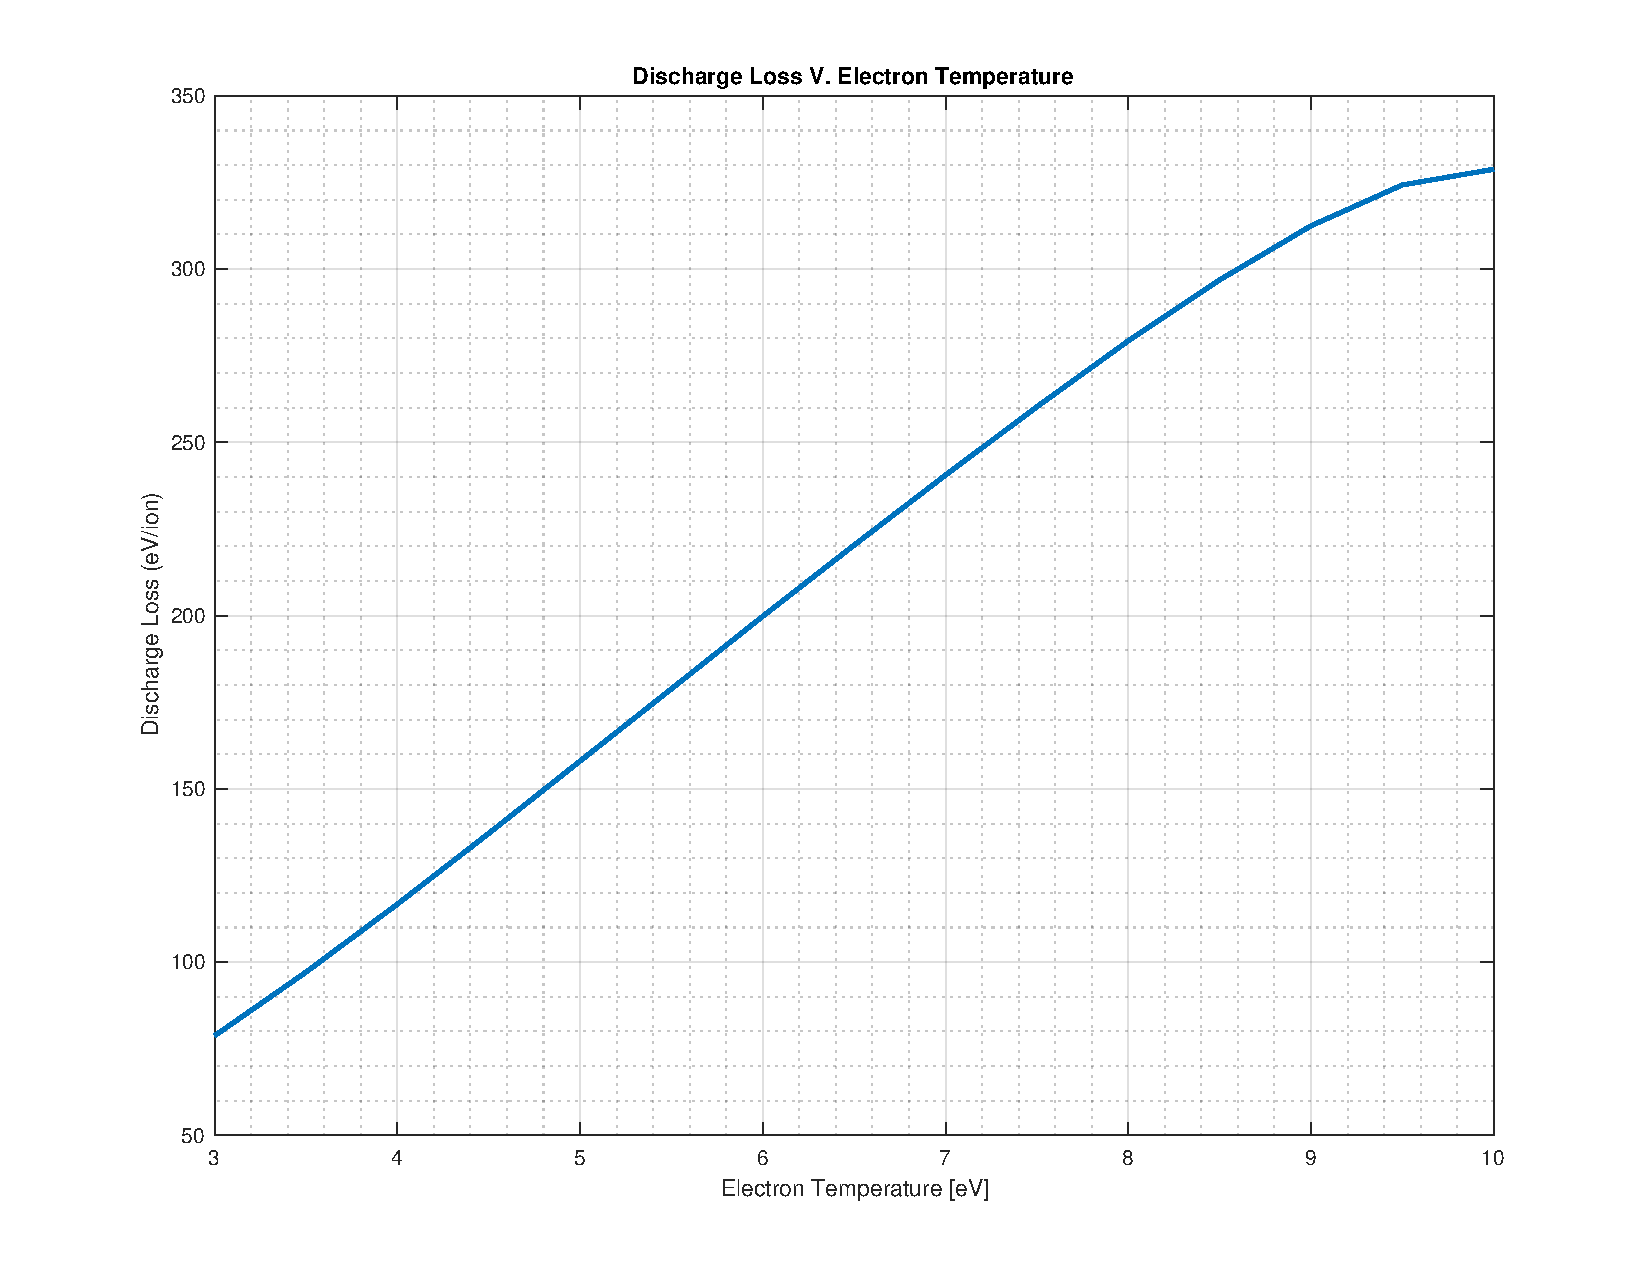
\includepdf{Problem1.pdf}
\newpage
\begin{lstlisting}
function hw8p2
clc;clear;

M = 2.18e-25;   % Ion Mass [kg]
n_o = 10^13 * (1/1e-6); %Beutral Xenon Gass Density [m^-3]
Volume = 10^4*1e-6; % Plasma Volume [m^3]
Area = 200*0.0001; % Ion Loss Area [m^2]

k = 1.38064852e-23; % Boltzmann Constant [J/K]
k2 = 8.6173303e-5;  % Boltzmann Constant [eV/K]

K = (k/k2);
EE = (2*n_o*Volume)/Area;

OVi_low = 1.08e-16;
OVi_high = 1.2775e-16; % From Hand Calculations
Te_low = 2;
Te_high = 2.03125; % From Hand Calculations

%Assuming linear relation between ionization rates.
while Te_high-Te_low > .00000001
    ovi = (OVi_high+OVi_low)/2;
    t = (Te_high+Te_low)/2;
    Te_new = (EE^2 * ovi^2)*(M/K);
    if Te_new >= t
        OVi_high = ovi;
        Te_high = t;
    else
        OVi_low = ovi;
        Te_low = t;
    end
end

Te_guess = Te_low;
OVi = OVi_high
Te_calculated = (EE^2 * OVi^2)*(M/K)

end
\end{lstlisting}
\newpage
\begin{lstlisting}
function hw8p3
e = 1.60217662e-19; % Electron Charge [J]
r_inner = .10/2;    % Inner Radius [m]
r_outer = .15/2;    % Outer Radius [m]
Ae = (pi*r_outer^2)-(pi*r_inner^2); % Exit Area [m^2]
ni = 5e17;      % Ion Plasma Density [m^-3]
B = 200;        % Radial Magnetic Field [G]
m =9.10938e-31; % Electron Mass [kg]
M = 2.18e-25;   % Ion Mass [kg]
Te = 20;        % Electron Temperature [eV]
Vd = 300;       % Discharge Champer Potential [V]

k = 1.38064852e-23; % Boltzmann Constant [J/K]
k2 = 8.6173303e-5;  % Boltzmann Constant [eV/K]

%Part A
Ii = ni*e * sqrt((2*e*Vd)/(M))*Ae;  % Beam Current [A]
P = Ii*Vd;                          % Beam Power [W]

%Part B
r_L = ((m*1000)/(e*B))*sqrt((8*(k/k2)*Te)/(pi*m))*1000*10; % Larmor Radius [mm]

%Part C
wB = (e*B)/(m);                     % Cyclotron Frequency [1/s]
Q = 6.5e-13/((3/2)*Te)^2;           % Collisional Cross Section
vth = sqrt((8*(k/k2)*Te)/(pi*m));   % Collision Speed
nu = ni*Q*vth;                      % Collision Frequency [1/s]

omega = sqrt(wB^2/nu^2); % Hall Parameter

%Part D
gamma= 0.9;     % Thrust Coefficient Factor
eta_m = 0.8;    % Mass Utilization Efficiency


mdot_i = (Ii*M)/e;
vi = sqrt((2*e*Vd)/(M));
Isp = (gamma*eta_m*vi)/9.81;
T = gamma*mdot_i*vi;

%Part E
IH = ni*e*((.15-.1)/2)*(Vd/(B*10^-4));
I_H = (Ii/(2*pi*((r_inner+r_outer)/2)*(B*10^-4)))*sqrt((M*Vd)/(2*e));
end
\end{lstlisting}

\newpage
\begin{lstlisting}
function hw8p5
m =9.10938e-31;
M = 2.18e-25;           % Ion Mass [kg]
k = 1.3806e-23;         % Boltzmann Constant [J/K]
k2 = 8.6173e-5;         % Boltzmann Constant [eV/K]
K = (k/k2);             % Boltzmann Constant [J/eV]
n_o = 10^13 * (1/1e-6); % Neutral Xenon Gas Density [m^-3]
Volume = 10^4*1e-6;     % Plasma Volume [m^3]
Area = 200*0.0001;      % Ion Loss Area [m^2]
EE = (2*n_o*Volume)/Area;
eo = 8.854e-12;         % Vacuum Dielectric Constant [C^2/Nm^2]
h = 6.6262e-34;         % Planks Constant [Js]
qe = 1.60217662e-19;    % Electron Charge [C]
ao = (eo*h^2)/(pi*m*qe^2);  % Atomic Cross Section [m^2]
Q = pi*ao^2*4.38;           % Emperical Cross Section [m^2]
%% This approach uses equations fitted to the empiracle ionization distributions to calculate the maxwellian distribution given a specific value of Te.
Te_low = 1; 	Te_high = 3;
while Te_high-Te_low > .0000000000001
    Te = (Te_low+Te_high)/2;
    if Te < 5
        %Maxwellian Ionization Rate Coefficient
        MOVi = 10^-20*((3.97+0.643*Te - 0.0368*Te^2)*exp(-12.127/Te))*sqrt((8*K*Te)/(pi*m));
    else
        %Maxwellian Ionization Rate Coefficient
        MOVi = 10^-20*(-(1.031e-4*Te^2) + 6.386*exp(-12.127/Te))*sqrt((8*K*Te)/(pi*m));
    end
    Vth = sqrt((8*K*Te)/(pi*m));
    OVi = 0.0005*Q*Vth + 0.9995*MOVi;
    Te_new = (EE^2 * OVi^2)*(M/K);
    if Te_new >= Te
        Te_high = Te;
    else
        Te_low = Te;
    end
end
%% This approach assumes a linear relation between the maxwellian ionizaion reaction rates and solves for a new ionization coefficient rate. With this,Te is recalculated and compared to the guessed Te value.
Te_low = 1.5; 	Te_high = 2; 	OVi_low = 1.16e-17; 	OVi_high = 1.08e-16;
while Te_high-Te_low > .000000000001
    ovi = (OVi_high+OVi_low)/2;
    t = (Te_high+Te_low)/2;
    Vth = sqrt((8*K*Te)/(pi*m));
    OVI = 0.0005*Q*Vth + 0.9995*ovi;
    Te_new = (EE^2 * OVI^2)*(M/K);
    if Te_new >= t
        OVi_high = ovi;
        Te_high = t;
    else
        OVi_low = ovi;
        Te_low = t;
    end	end	end
\end{lstlisting}

\end{document}